\documentclass{article} % Класс печатного документа

\usepackage{hyperref} % Для вставки гиперссылок
\usepackage{listings} % Для вставки кусков кода
\usepackage{graphicx} % Вставка изображений
\usepackage[utf8]{inputenc} % Кодировка исходного текста - utf8
\usepackage[english,russian]{babel} % Поддержка языка - русского с английским
\usepackage{indentfirst} % Отступ в первом абзаце

\title{Отчёт 1\protect\\Кластерный анализ} % Заголовок документа
\author{Свичкарев А.\,В.} % Автор документа
\date{\today} % Текущая дата

\begin{document} % Конец преамбулы, начало текста

\maketitle % Печатает заголовок, список авторов и дату

\section{Цель}
Изучить способы решения задач поиска кластеров в данных.

\section{Задание №1}
Написать программу формирования данных случайных кластеров и
их кластерного анализа по алгоритму <<associative clustering>> с пороговым значением 0.12.
Визуализировать в виде графика и сохранить файл изображения графика кластеров.

\clearpage

Реализация взята из Приложения, произведён рефакторинг и разобран алгоритм.
Выборки для разных алгоритмов были одинаков, чтобы можно было провести сравнение.

\noindent\makebox[\textwidth]{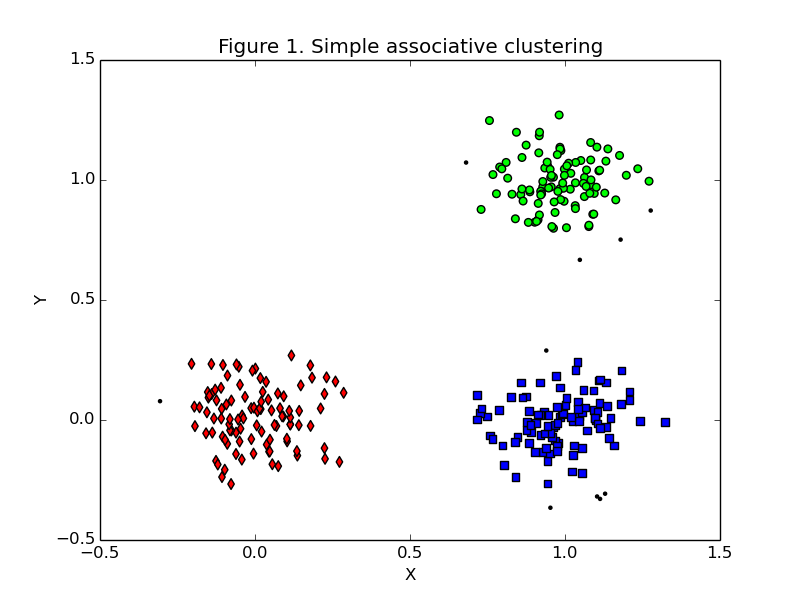
\includegraphics[width=0.7\paperwidth]{Figure_1}}

В разделе приложения представлено две разновидности алгоритма:
простой алгоритм кластеризации и вариант с очистрой от шума.

Для обоих вариантах вначале вычисляется матрица попарных расстояний в эвклидовой метрике между всеми вершинами.
Если расстояние меньше заданного порога, то вершины считаются соседними.
Основной шаг формирования кластеров заключается в слиянии всех вершин, являющихся соседями.
Слияние продолжается также по транзитивности,
т.е. если вершина А является соседней к B,
а B к C, то C считается соседом A и добавляется в кластер.
Кластер считается заполненным, когда кончаются соседи.
Благодаря транзитивности алгоритм работает быстро,
однако такая транзитивность не всегда может вести к хорошим результатам.

Второй вариант алгоритма аналогичен,
только к нему добавляются проверки числа соседей для вершин.
Если соседей вершины меньше порога, то она считается выбросом - шумом.

\clearpage

Выделенные кластера без шума:

\noindent\makebox[\textwidth]{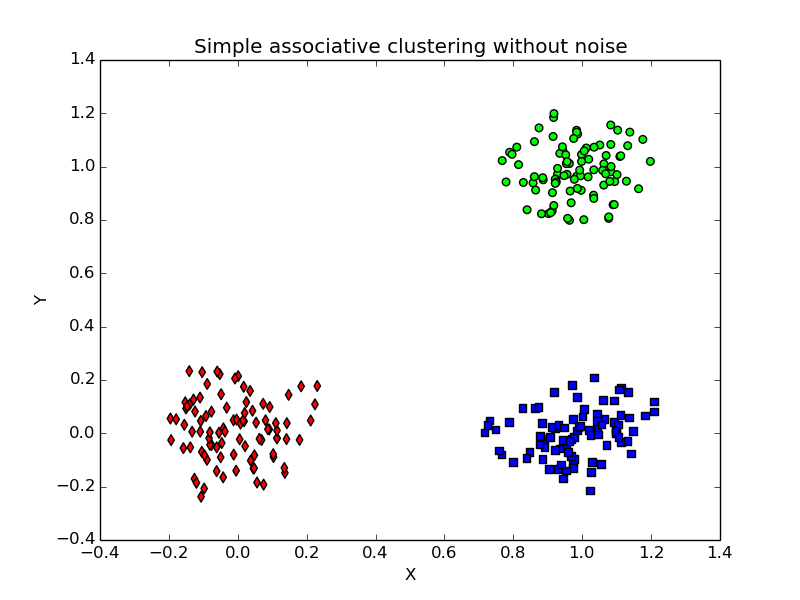
\includegraphics[width=0.7\paperwidth]{Figure_4}}

В секции Исходный код представлена реализация.

\section{Задание №2}

Написать программу визуализации кластеров в виде «дендрограммы» и сохранить
дендограмму в виде файла изображения.

Была найдена статья по данной тематике в Интернете
\href{https://joernhees.de/blog/2015/08/26/scipy-hierarchical-clustering-and-dendrogram-tutorial/}
{SciPy Hierarchical Clustering and Dendrogram Tutorial}
В данной статье была разобрана кластеризация с использованием библиотеки scipy.

Для проведения кластеризации использовалась функция \textit{linkage()}.
В отличие от реализации из Приложения,
здесь использовался другой подход,
где объединение в кластер происходило всегда самых ближайших кластеров.
Это можно проследить, проанализировав вывод первых 20 объединений в кластера.
Видно, что расстояния постепенно увеличиваются.

На следующем изображение представлена кластеризация на той же выборке, что и для Задания 1:

\noindent\makebox[\textwidth]{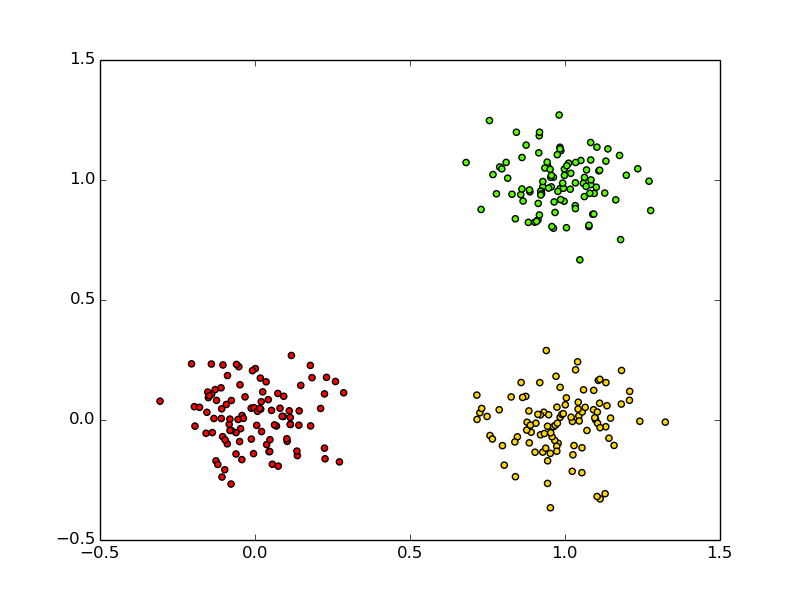
\includegraphics[width=0.7\paperwidth]{Figure_2}}

\clearpage

Удобство использования функции \textit{linkage()} заключается в информативном выходном значение,
которое содержит массив исходных вершин и итеративное построение новых кластеров с указанием расстояния.
Чтобы построить дендрограмму, достаточно вызвать функцию \textit{dendrogram()}:

\noindent\makebox[\textwidth]{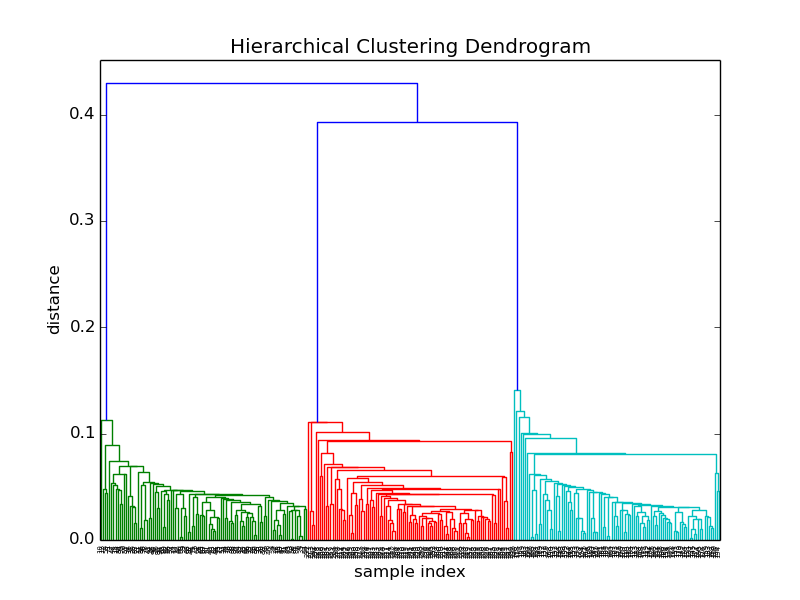
\includegraphics[width=0.7\paperwidth]{Figure_3}}

\section{Пояснение}
Исходный код доступен по ссылке:
\href{https://github.com/SvichkarevAnatoly/Course-Python-Bioinformatics/tree/master/bioseq7}
{github.com}

\clearpage

\section{Исходный код}
Файл \verb$example.py$:
\lstinputlisting[language=Python]{../example.py}

Файл \verb$dendrogram.py$:
\lstinputlisting[language=Python]{../dendrogram.py}

\end{document} % Конец документа
